% Stay on Task: final report. Build with: sh compile.sh (pdflatex), tectonic report.tex, or upload this folder to Overleaf
\documentclass[10pt,a4paper]{article}
\usepackage[T1]{fontenc}
\usepackage[utf8]{inputenc}
\usepackage{tgtermes}
\usepackage[scale=0.9]{tgheros}
\usepackage[scale=0.88]{tgcursor}
\usepackage{microtype}
\usepackage[a4paper,top=20mm,bottom=19mm,left=19mm,right=19mm,headheight=13pt]{geometry}
\usepackage[table]{xcolor}
\usepackage{graphicx,booktabs,tabularx,array,enumitem,float,amsmath,fancyhdr,lastpage,titlesec,needspace}
\usepackage[font=small,labelfont=bf,labelsep=period,skip=3pt]{caption}
\usepackage{xltabular}
\usepackage[hidelinks]{hyperref}

\definecolor{head}{gray}{0.12}
\definecolor{sub}{gray}{0.35}
\definecolor{rule}{gray}{0.55}
\definecolor{shade}{gray}{0.95}
\definecolor{rowshade}{gray}{0.955}
\definecolor{accent}{HTML}{2F5D8A}
\definecolor{boxbg}{HTML}{EEF3F9}
\hypersetup{colorlinks=true,linkcolor=accent,urlcolor=accent,citecolor=accent}

\titleformat{\section}{\needspace{8\baselineskip}\sffamily\large\bfseries\color{accent}}{\thesection}{0.6em}{}[{\color{rule}\titlerule[0.5pt]}]
\titleformat{\subsection}{\needspace{5\baselineskip}\sffamily\normalsize\bfseries\color{head}}{\thesubsection}{0.6em}{}
\titlespacing*{\section}{0pt}{10pt}{4pt}
\titlespacing*{\subsection}{0pt}{6pt}{2pt}

\pagestyle{fancy}
\fancyhf{}
\fancyhead[L]{\small\sffamily\color{sub}Stay on Task: final report}
\fancyhead[R]{\small\sffamily\color{sub}LMA Group Project 2026}
\fancyfoot[C]{\small\sffamily\color{sub}\thepage\ of \pageref{LastPage}}
\renewcommand{\headrulewidth}{0.3pt}
\fancypagestyle{plain}{\fancyhf{}\renewcommand{\headrulewidth}{0pt}\fancyfoot[C]{\small\sffamily\color{sub}\thepage\ of \pageref{LastPage}}}

\setlist{itemsep=1pt,topsep=2pt,parsep=0pt,leftmargin=13pt}
\setlength{\parindent}{0pt}
\setlength{\parskip}{4pt}
\renewcommand{\arraystretch}{1.15}
\newcolumntype{Y}{>{\raggedright\arraybackslash}X}
\newcolumntype{P}[1]{>{\raggedright\arraybackslash}p{#1}}
\newcommand{\tablestyle}{\footnotesize\rowcolors{2}{rowshade}{white}}
\newcommand{\code}[1]{\texttt{#1}}
\newcommand{\m}{$-$}

\begin{document}

\thispagestyle{plain}
\begin{center}
{\color{rule}\rule{\linewidth}{1.2pt}}\\[4pt]
{\small\sffamily\color{sub}LMA Group Project 2026 \enspace\textperiodcentered\enspace Final report \enspace\textperiodcentered\enspace November 2026}\\[5pt]
{\sffamily\LARGE\bfseries\color{head} Stay on Task: can a small classifier\\[1pt] correct local agents' drift?}\\[7pt]
\begin{tabular}{cccc}
\textbf{Shuban Biswas} & \textbf{Ch Pavan Harshit} & \textbf{Swayam Goyal} & \textbf{Aaditya Sharma}\\
{\footnotesize 2024111017} & {\footnotesize 2025701057} & {\footnotesize 2024111012} & {\footnotesize 2019113009}
\end{tabular}\\[4pt]
{\footnotesize Code, data, results and reproduction guide: \url{https://github.com/ch-pavan/lma-grp-project}}\\[2pt]
{\color{rule}\rule{\linewidth}{0.5pt}}
\end{center}

\section*{Abstract}
Small local agents drift off task, leave requests unfinished and claim work they did not do. The usual fix, a small language model (SLM) judge that reasons before every step, is slow and expensive. We ask whether a 0.4B classifier, Laya, finetuned for the job, can take the judge's place. Our agent is Qwen3.5 9B on the BFCL v4 multi turn benchmark, inside a planner and doer harness with rollback and a turn end ``done check''. On 1,200 held out test tasks, Laya raises the pass rate from 45.5\% to 49.2\% (+3.7 points [+0.8, +6.8]). That is exactly the gain of a reasoning Qwen3.5 9B judge (Laya minus judge +0.0 [\m2.8, +2.9]), at zero judge tokens against 52.7k per task and a third of the judge's time per task. Offline, on 7,214 test steps labelled by two LLM annotators, a three way closing message head (done, off track, false claim) beats the 9B judge on the proposal's primary metric by 13 to 19 F1 points. Every 95\% interval is above zero, clearing our 9 point bar. That head was designed after our pre-test freeze. The frozen two head design falls 17 points short, because it cannot call an unfinished closing message off track, and this diagnosis is what led to the three way head. We release the harness, a replay oracle that labels every step automatically, over 12,700 LLM labelled steps (checked by hand on a 200 step sample), and every run.

\begin{table}[H]
\centering\tablestyle
\caption{Headline results. Intervals are 95\% bootstrap over scenarios, paired for differences.}\label{tab:headline}
\begin{tabularx}{\linewidth}{P{0.36\linewidth}Y}
\toprule
\textbf{Question} & \textbf{Result} \\
\midrule
Task accuracy on test, rollback plus done check & Laya 49.2\% and 9B SLM judge 49.2\%, both +3.7 over no judge with the interval above zero. Laya minus judge +0.0 [\m2.8, +2.9]. \\
Cost of the check & Laya: 0 judge tokens, 528 s per task. 9B judge: 52,672 judge tokens and 1,621 s per task. \\
Detection on 7,214 test steps (primary F1) & Typed Laya 0.38 to 0.44 against 0.24 to 0.25 for the 9B judge: +13.1 to +19.0 points, intervals above zero. Frozen Laya 0.06 to 0.08. \\
Off track closing messages (F1) & Typed Laya 0.65 to 0.72 against 0.27 to 0.29 for the 9B judge. \\
Off track tool calls (F1) & Laya 0.23 to 0.28 against 0.17 to 0.21 for the 9B judge, on test. \\
Label quality & Annotators against our human check: kappa 0.84 and 0.71. Between the annotators on test: kappa 0.55 to 0.57. \\
\bottomrule
\end{tabularx}
\end{table}

\section{Introduction}\label{sec:intro}
Agents built on small open models can run on a normal computer and act through tools: files, messages, posts, bookings and trading accounts. A user who wants this private and cheap cannot send every step to a large cloud model. But partway through a task, small agents lose track of the request, make up values, stop early and report success they did not achieve. The standard remedy is an SLM judge that checks each step before it runs~\cite{zheng2023judge}. A small model judging itself is weak~\cite{critictool}, and a judge that reasons for 1,500 to 2,400 tokens per step multiplies the cost of every task. Tiny monitors have so far struggled on real, unplanned mistakes~\cite{realtime}.

\textbf{Research question.} Can a finetuned small classifier, given the same state as an SLM judge, detect off track steps and false claims better than that judge, and what does it do to task accuracy and cost?

\textbf{Hypothesis and falsification rule (fixed in the proposal).} The primary metric is the mean F1 of off track steps and false claims against labels from two LLM annotators. The classifier must beat the SLM judge by at least 9 F1 points, with the 95\% interval above zero. For task accuracy, the full system should beat no judge and stay within 5 points of the SLM judge baseline, at a fraction of its judge tokens.

\textbf{Contributions.}
\begin{itemize}
  \item \textbf{The first per question comparison of a sub 1B judge with an SLM judge}, offline on the same states and live inside the same agent.
  \item \textbf{A cheap check that matches the SLM judge live.} Laya, one forward pass of a 0.4B encoder per check, gives the same +3.7 point test gain as a reasoning 9B judge, at zero judge tokens and a third of the time per task (Section~\ref{sec:eval-live}).
  \item \textbf{A typed closing message head that beats the SLM judge on detection} by 13 to 19 F1 points on 7,214 test steps, above the proposal's 9 point bar (Section~\ref{sec:eval-primary}).
  \item \textbf{A diagnosis of where step checks fail.} Most errors of a capable small agent are unfinished turns, which a step check cannot see. 64\% of failed test tasks end in a stopped, needlessly asking or falsely ``done'' turn (Section~\ref{sec:eval-fail}).
  \item \textbf{Resources.} A cleaned BFCL split with an empty turn check, a replay oracle that labels every step, a guide-based LLM annotation pipeline checked by humans, and over 12,700 labelled steps. Everything runs from the repository (Section~\ref{sec:repo}).
\end{itemize}

\section{Literature review}\label{sec:lit}
\textbf{Step guards.} Existing guards are 0.8B to 8B generative safety models that \emph{block} a step rather than correct it: Granite Guardian~\cite{granite}, StepGuard~\cite{stepguard}, SAFETY SENTRY~\cite{sentry} and AgentDoG~\cite{agentdog}. Each targets harmful or risky actions, not a step that is safe but off task.

\textbf{Narrow small checkers.} Small models check one risk each: function call hallucination (Granite Guardian's function call risk~\cite{granite}), unsupported claims (MiniCheck~\cite{minicheck}, Vectara HHEM~\cite{hhem}, LettuceDetect~\cite{lettuce}) and injected instructions (LlamaFirewall and PromptGuard~\cite{llamafirewall}). Kev 0.8B~\cite{kev} is an open Jev style model~\cite{typesafe} that scores below chance on When2Call~\cite{when2call} by its own card. We use it as a reference point.

\textbf{Reward models and judges.} Step reward models such as ToolRM~\cite{toolrm} and AgentPRM~\cite{agentprm} rank candidate steps for best of N picking. Math-Shepherd~\cite{mathshepherd} labels steps automatically by whether a correct ending is still reachable, the idea behind our replay oracle. LLM as a judge~\cite{zheng2023judge} is the standard baseline. CRITICTOOL~\cite{critictool} shows small models critique their own tool calls poorly. Cascades that send only uncertain inputs to a larger model cut cost~\cite{frugalgpt}.

\textbf{Typed decision classifiers.} Laya~\cite{laya} is a 0.4B ModernBERT~\cite{modernbert} model that answers typed questions (choice, yes/no) in one forward pass, in the Jev style~\cite{typesafe}. A Laya head already picks actions in a browser agent~\cite{layabrowser}.

\textbf{Benchmarks.} BFCL v4 multi turn~\cite{bfcl} grades agents on the end state of simulated apps, but some tasks have unsound answer keys~\cite{bfclissues}. AgentDojo~\cite{agentdojo} checks utility in four realistic suites. $\tau^2$-bench is excluded because an agent that does nothing passes 23 of its 50 airline tasks~\cite{tau2}. AgentProcessBench~\cite{agentprocessbench} and AgentHallu~\cite{agenthallu} label wrong steps of agent traces.

\textbf{The gap.} We found no work that uses a sub 1B classifier as the judge of a multi agent pipeline and compares it, question by question and live, with an SLM judge given the same state. That is the comparison this project makes.

\section{Datasets created and used}\label{sec:data}
Table~\ref{tab:data} lists every task set, recorded run and label set we built or used; Table~\ref{tab:balance} gives the class balance.
\begin{table}[htbp]
\centering\tablestyle
\caption{Task sets, recorded runs and labels. Every row is in the repository.}\label{tab:data}
\begin{tabularx}{\linewidth}{P{0.24\linewidth}Y}
\toprule
\textbf{BFCL v4 multi turn, cleaned} & 200 scenarios in 4 versions (base, missing parameter, missing function, long context), 8 simulated apps. 11 unsound scenarios dropped~\cite{bfclissues}, split by scenario into 74 train, 15 validation and 100 test. Pass = BFCL's state checker plus our empty turn check: any state change on a turn whose correct answer is to call nothing fails. \\
\textbf{AgentDojo benign} & 97 user tasks (workspace, travel, banking, Slack), no injections, the suite's own utility check. Outside check only, never used for training or tuning. \\
\textbf{9B runs, train and validation} & Train 888 tasks (8,806 calls, 3,737 turn ends). Validation 120 tasks (1,277 calls, 495 turn ends), plus 120 with reasoning on. \\
\textbf{8B runs} & 356 Qwen3 8B tasks on train and validation scenarios (3,824 steps), pooled into the step head's training data, plus 3,635 gold replay steps. \\
\textbf{9B test passes} & 8 passes of the 400 test tasks with no judge, every step's judge input recorded: 3,200 tasks, 29,520 calls, 12,963 closing messages. A further 1,200 recorded tasks on Ada pair with the live runs. \\
\textbf{Test sample} & 7,214 steps (5,171 calls, 2,043 closing messages) by the proposal's rule: failed turns in random order up to their first off track call, then 500 passed turn steps. \\
\textbf{Laya training sets} & Step head: 8,847 train, 1,975 dev, 2,427 validation calls (408, 55 and 186 bad). Done head: 3,341 train, 396 dev, 495 validation turn ends (622, 50 and 111 not done). Typed head: all 3,737 train closing messages with annotator labels. Split by scenario; no test scenario is in any training set. \\
\bottomrule
\end{tabularx}
\end{table}

\textbf{Automatic labels: a replay oracle.} After each call, the oracle replays every order-kept subset of the turn's reference calls as a possible ending. The first call after which no ending reaches the reference state is \emph{off track}. A closing message with success words while the state is wrong is a \emph{false claim}. A turn is \emph{done} if its end state matches the reference and every reference function was called. Gold replay passes 755 of 756 BFCL tasks and 97 of 97 AgentDojo tasks, so the harness and oracle are sound.

\textbf{LLM annotators.} Annotator A is DeepSeek V4.1 Flash~\cite{deepseek} and Annotator B is GLM-5.3-Flash~\cite{glm}, from two model families, neither Qwen nor Gemma, so no judge under test grades its own errors. They follow a written guide, following the guidelines for empirical studies with LLMs~\cite{baltes}, and see neither the oracle labels nor the BFCL verdict. A tool call gets Q1 (on or off track) and Q2 (none or made up value). A closing message gets one typed answer: done, missing action, should ask user, or unsupported claim. Labelled: all 1,772 validation steps (guide v2), the 200 human check steps (guide v3), the 7,214 test steps (guide v3) and the 3,737 train closing messages (guide v3), 12,723 steps in all.

\begin{table}[H]
\centering\tablestyle
\caption{Class balance. Train and validation: replay oracle labels on the 9B runs. Test: the 7,214 step sample, labels from Annotator A / B / both agree.}\label{tab:balance}
\begin{tabularx}{\linewidth}{Yccc}
\toprule
\textbf{Class} & \textbf{Train} & \textbf{Validation} & \textbf{Test sample} \\
\midrule
Off track (tool calls) & 221 of 8,806 (2.5\%) & 63 of 1,277 (4.9\%) & 162 / 210 / 108 of 5,171 \\
Off track (closing messages) & & & 980 / 805 / 667 of 2,043 \\
False claim (closing messages) & 281 of 3,737 (7.5\%) & 50 of 495 (10.1\%) & 91 / 76 / 49 of 2,043 \\
Turn not done & 672 of 3,737 (18.0\%) & 111 of 495 (22.4\%) & \\
\bottomrule
\end{tabularx}
\end{table}
Every class is rare, so we report per class precision, recall and F1 (never accuracy), train with balanced class weights and choose thresholds by F1 on out-of-fold scores.

\textbf{Gate 1 class counts.} Pooled over the 9B and 8B training scenarios, off track (310) and false claim (372) pass the proposal's 300 example gate, so both primary classes are trainable. Unneeded irreversible calls (217) and made up values (at most 143) do not, so they are folded into the step head rather than trained as separate questions.

\section{Methodology}\label{sec:method}
\subsection{Agent and harness}
For each user turn a planner writes a short plan and a doer makes tool calls with Qwen3.5 9B~\cite{qwen} (4 bit AWQ, reasoning off, vLLM, 32k context). A checker sits in two places (Figure~\ref{fig:system}):
\begin{itemize}
  \item \textbf{Step check, before each tool call runs.} If the call is bad, it is rolled back and the doer resamples it, at most twice.
  \item \textbf{Done check, when the doer ends a turn.} If the turn is not done, the closing message is dropped and the agent is told part of the request may be unfinished, at most twice per turn.
\end{itemize}
This correction mode (\code{rbh2dc}) won the correction action study (Section~\ref{sec:ablations}). Code handles what needs no model: exact repeats of a failed call, the fixed list of irreversible tools and the evidence list, which says where each argument value appears.

\begin{figure}[H]
\centering
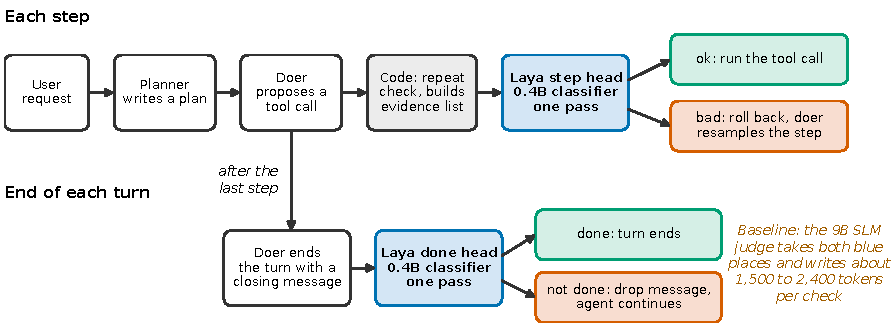
\includegraphics[width=0.93\linewidth]{figs/fig1_system.pdf}
\caption{System. The blue boxes are the two Laya checks. In the baseline, the 9B SLM judge sits in both places and reasons before each answer. In the typed variant, the done head is replaced by a three way head (done, off track, false claim).}\label{fig:system}
\end{figure}

\subsection{The checkers compared}
\begin{itemize}
  \item \textbf{S1 no judge.}
  \item \textbf{S2 plain rules.} A value without evidence is made up, a success word without a successful call is a false claim, a call outside the plan is drift, and every irreversible call asks the user.
  \item \textbf{S3 SLM judge.} The same 9B model with reasoning on, given the same state and guide.
  \item \textbf{Off the shelf judges.} Laya as is, Granite Guardian 3.2 3B A800M~\cite{granite}, Kev 0.8B~\cite{kev}, LettuceDetect~\cite{lettuce}.
  \item \textbf{Laya finetuned.} The checker under test.
  \item \textbf{Oracle.} Flags exactly the steps the replay oracle marks: a ceiling that has the answer key and cannot be deployed.
\end{itemize}

\subsection{Laya heads}
Laya~\cite{laya} (0.3.27, revision \code{e929ae5}) reads a state of up to 1,024 tokens. The state puts the most important text first, since Laya cuts the end of a long input. For a call: the proposed call, the evidence list, the latest request, the last calls with outputs cut short, the plan and earlier requests. For a closing message: the message, the latest request, this turn's calls newest first, and earlier requests. Each head is one typed choice question, fully finetuned with balanced class weights, option order shuffled per example, encoder learning rate $2\times10^{-5}$ and head learning rate $10^{-4}$.
\begin{itemize}
  \item \textbf{Step head (ok / bad).} Trained on oracle labels: bad = breaks the task, an unneeded irreversible call, or a made up value in an irreversible call. 16 minutes on an RTX 6000 Ada, about 50 on an RTX 2080 Ti.
  \item \textbf{Done head (done / not done).} Trained on oracle labels at turn ends. 5 to 9 minutes.
  \item \textbf{Typed closing message head (done / off track / false claim).} Trained on the average of the two annotators' guide v3 labels, used as a soft target, for the 3,737 train closing messages. Off track = missing action or should ask user; false claim = unsupported claim. The decision rule is: false claim if $P(\text{fc}) \ge 0.260$, else off track if $P(\text{off}) \ge 0.417$, else done. Both thresholds come from 5 scenario-grouped folds of train, out of fold. 2 epochs, under 3 minutes per run on a 40 GB GPU. Its training labels hold 182 false claims marked by either annotator (56 by both) and 630 off track closing messages (293 by both). Before training, Laya as is reproduced its Ada result in the new environment (dev AUROC 0.751 against 0.752).
\end{itemize}

\subsection{Metrics and protocol}
\textbf{Detection.} Per class precision, recall and F1, with AUROC for the heads. The primary metric is the mean F1 of off track (Q1, on calls and closing messages) and false claim (Q2, on closing messages), scored against Annotator A, Annotator B, and the steps where both agree. A false claim closing message counts as on track for Q1. Any other unfinished turn counts as off track.

\textbf{Task accuracy.} The share of 1,200 test tasks passed (100 scenarios $\times$ 4 versions $\times$ 3 runs). Differences use a paired bootstrap over the 100 scenarios. We also report judge tokens and seconds per task.

\textbf{Fixed before looking.} The step head (Ada seed \code{orig\_seed1}, best of 3 seeds on dev, threshold 0.1266) and done head (threshold 0.561, out of fold on train) were frozen on 8 November, before any test run with Laya. The typed head's every choice was written down on 9 November before training, and the test set was scored once, after the run was chosen on validation. All thresholds come from train or dev, never from validation or test.

\subsection{Changes from the proposal and response to feedback}\label{sec:changes}
\begin{itemize}
  \item \textbf{Agent and checker design.} Block and warn became rollback plus a done check, after the correction action study (Section~\ref{sec:ablations}). Q3 (needed irreversible call) is folded into the step head, since unneeded irreversible calls (217) missed Gate 1. The binary done head was extended to the typed closing message head, which answers Q1 and Q2 at turn end.
  \item \textbf{Training data.} The directed runs with Qwen3.8 27B were dropped by team decision (24 October). The step head trains on natural mistakes of Qwen3.5 9B and Qwen3 8B, and the 8B steps stand in for the planned 4B pass.
  \item \textbf{Test passes.} The stop rule ``300 false claims or 8 passes'' ended at 8 passes. GLM-5.3-Flash is used in place of GLM-5.3. Turing became unavailable, so the 9B test ran on Ada and on a rented GPU, each paired with its own no judge run.
  \item \textbf{Feedback on the proposal.} We report the class distribution (Table~\ref{tab:balance}), finetuning gain per head and per class against as is and against plain rules, and the correction action ablation (Section~\ref{sec:ablations}). On the contest between the classifier and the judge, we report off track on calls and on closing messages and false claims separately (Figure~\ref{fig:primary}b). The state component ablation was not run (Section~\ref{sec:limits}).
\end{itemize}

\section{Experiment runs}\label{sec:experiments}
\subsection{Choosing the agent}
\begin{figure}[H]
\centering
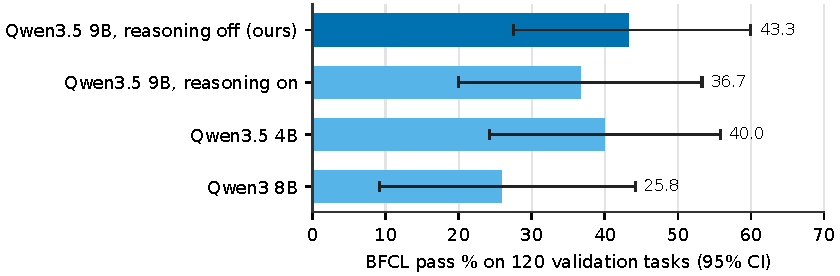
\includegraphics[width=0.55\linewidth]{figs/fig2_agents.pdf}
\caption{Agent models on the same 120 validation tasks. Qwen3.5 9B with reasoning off is our agent.}\label{fig:agents}
\end{figure}
Qwen3.5 4B passes 40.0\% against 25.8\% for Qwen3 8B, so model generation matters more than size. The 9B passes 43.3\% on validation and 52.7\% [44.8, 60.5] on train. Turning reasoning on costs 6.6 points and 2.5 times the time, so the agent runs with reasoning off.

\subsection{Baselines on the original Qwen3 8B test}
\begin{table}[H]
\centering\tablestyle
\caption{BFCL test, Qwen3 8B agent and judge, plain block mode, 100 scenarios $\times$ 4 versions $\times$ 3 runs. AgentDojo: 97 tasks $\times$ 3 runs.}\label{tab:test8b}
\begin{tabularx}{\linewidth}{Yrllrr}
\toprule
\textbf{System} & \textbf{Runs} & \textbf{BFCL pass \% [95\% CI]} & \textbf{vs S1 [95\% CI]} & \textbf{AgentDojo} & \textbf{s / task} \\
\midrule
S1 no judge & 1,200 & 15.9 [11.7, 20.5] & & 33.7 & 93 \\
S2 plain rules & 1,200 & 7.6 [4.4, 11.2] & \m8.3 [\m11.8, \m5.2] & 18.2 & 108 \\
S3 SLM judge (Qwen3 8B) & 1,200 & 17.4 [12.8, 22.3] & +1.5 [\m0.6, +3.8] & 25.8 & 202 \\
S4a Laya as is & 133, stopped & 0 (upper bound 2.2) & & & 336 \\
S4b Granite Guardian & 20 task pilot & 0 & & & \\
Laya finetuned, frozen & 1,200 & 13.5 [9.7, 17.8] & \m2.4 [\m5.2, +0.2] & & \\
\bottomrule
\end{tabularx}
\end{table}
\begin{figure}[H]
\centering
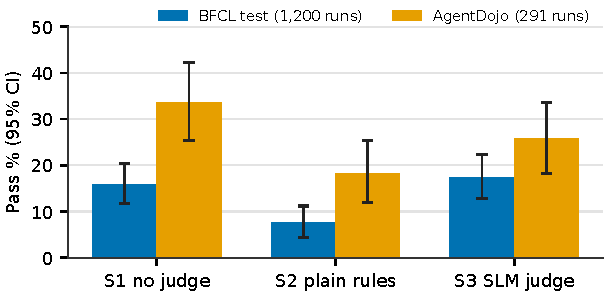
\includegraphics[width=0.6\linewidth]{figs/fig3_test_baselines.pdf}
\caption{Pass rates on BFCL test and AgentDojo (Qwen3 8B agent), 95\% confidence intervals.}\label{fig:test8b}
\end{figure}
Off the shelf, no small judge is usable. Laya as is blocked 87.6\% of judged steps, and Granite Guardian called all 169 calls it saw risky, so every run hit the step cap. Plain rules block good calls and cost 8.3 points. In plain block mode, finetuned Laya is within noise of no judge (\m2.4 [\m5.2, +0.2]) and below the 8B judge (\m3.9 [\m7.1, \m1.1]). Plain mode asks the done head again on every retry of a flagged closing message, so 596 of the 1,200 tasks run into the 20 step cap. The 9B system's rollback mode, with at most two done checks per turn, avoids this loop, and there Laya turns into a gain (Section~\ref{sec:eval-live}).

\subsection{Off the shelf judges, offline}
\begin{table}[H]
\centering\tablestyle
\caption{Primary score (mean F1 of off track and false claim) on the 1,772 validation steps of the 9B agent, guide v1 labels.}\label{tab:offline}
\begin{tabularx}{\linewidth}{Yccc}
\toprule
\textbf{Judge} & \textbf{vs oracle} & \textbf{vs Annotator A} & \textbf{vs Annotator B} \\
\midrule
Plain rules & 0.07 & 0.10 & 0.11 \\
Laya as is & 0.11 & 0.21 & 0.16 \\
Kev 0.8B & 0.15 & 0.12 & 0.07 \\
LettuceDetect (false claim only) & 0.18 & 0.22 & 0.15 \\
\bottomrule
\end{tabularx}
\end{table}
Laya as is stays at AUROC 0.39 to 0.67 across 4 state formats and 8 question wordings. Only the hosted Jev classifier showed signal, on closing messages (AUROC 0.81). Finetuning is needed.

\subsection{Finetuned Laya on validation}
\begin{figure}[H]
\centering
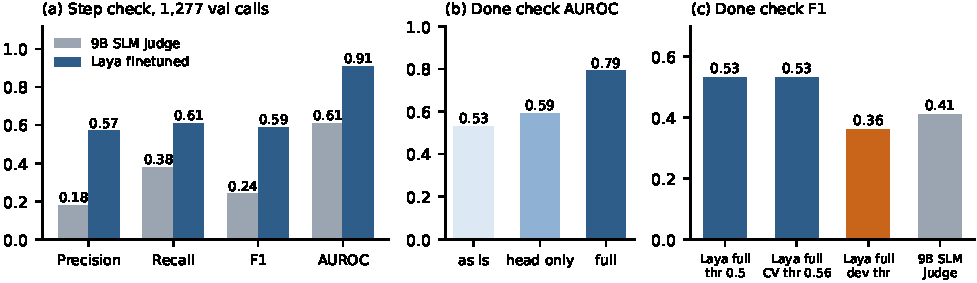
\includegraphics[width=\linewidth]{figs/fig_offline.pdf}
\caption{Finetuned Laya on validation. (a) Step check on 1,277 calls against the replay labels. (b, c) Done check on 495 turn ends against the oracle, positive class not done. Panel (c) shows Laya at threshold 0.5, at 0.56 from cross validation on train, and at the discarded dev threshold.}\label{fig:offlinelaya}
\end{figure}
\textbf{Step check.} Finetuning lifts AUROC from 0.57 as is to 0.90 on 2,427 pooled validation calls. On the 9B's 1,277 calls Laya scores F1 0.59 and AUROC 0.91, against 0.24 and 0.61 for the 9B judge. It beats ``flag every irreversible call'' on irreversible calls (AUROC 0.74 against 0.50) and also ranks reads (0.95), so it reads arguments and context, not just function names. Against the annotators with the judge on its own harness prompt, Laya leads on off track tool calls by +7.2 to +9.2 F1.

\textbf{Done check.} AUROC 0.79 against 0.53 as is and 0.59 for a head-only finetune. F1 is 0.53 at the train-chosen threshold against 0.41 for the 9B judge.

\textbf{Live on validation.} On 120 validation tasks no system differed from no judge beyond noise. Two identical no judge runs disagree on 28 of 120 tasks. The oracle's +4.2 [\m1.7, +10.8] showed how wide intervals are at this size, which is why the claim rests on the 1,200 task test set.

\textbf{Primary metric on validation, frozen design.} Laya minus the 9B judge is \m1.0 to +2.0 F1. The reason: the done head can only say ``not done'', which the proposal's scoring counts as a false claim. On validation that gives 105 to 108 false claim flags against 6 to 15 real false claims, and no off track flag on any closing message, even though the annotators mark 51 to 66 closing messages off track. This diagnosis, made on validation before any test run, is the motivation for the typed head.

\subsection{The test runs}
\begin{itemize}
  \item \textbf{No judge.} 8 passes on a rented 80 GB GPU (3,200 tasks, vLLM 0.27.1 as in validation): 46.5\% [40.4, 52.8]. 1,200 more tasks on Ada pair with the live runs: 45.5\% [39.2, 51.9].
  \item \textbf{Live, rollback plus done check, 1,200 tasks each.} Laya frozen, the 9B judge and the oracle ran on Ada with the 9B split over two RTX 2080 Ti cards. The typed head ran on the rented GPU, against the 3,200 no judge tasks served the same way.
  \item \textbf{Offline.} The 9B judge (harness prompt, reasoning on, 4,096 tokens, then a rejudge at 8,192 tokens, leaving 136 unparsed, 1.9\%), frozen Laya and typed Laya scored the 7,214 test steps, against both annotators' guide v3 labels.
\end{itemize}

\section{Ablations}\label{sec:ablations}
\begin{figure}[H]
\centering
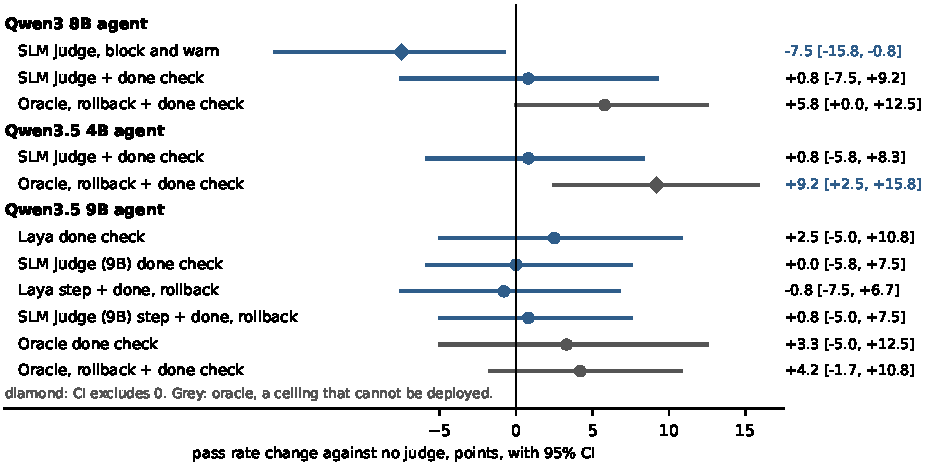
\includegraphics[width=0.95\linewidth]{figs/fig_forest.pdf}
\caption{Correction actions on validation: pass rate change against no judge (120 tasks per system). Rollback plus the done check is the only action that helps with the oracle on every agent, and it is the mode used on test.}\label{fig:forest}
\end{figure}

{\tablestyle
\begin{xltabular}{\linewidth}{P{0.24\linewidth}Y}
\caption{Ablations. Validation unless marked test.}\label{tab:ablations}\\
\toprule
\textbf{Ablation} & \textbf{Result} \\
\midrule
\endfirsthead
\toprule
\textbf{Ablation} & \textbf{Result} \\
\midrule
\endhead
Correction action (Qwen3 8B) & Block and warn does not help even with the oracle (+2.5 [\m1.7, +6.7]) and hurts with the SLM judge (18.3\% against 25.8\%). Rollback removes that damage (22.5 to 24.2\%). A vote of 3 does not help (\m5.0 [\m12.5, +1.7]). Rollback plus the done check with the oracle: +9.2 [+2.5, +15.8] on Qwen3.5 4B and +5.8 [0.0, +12.5] on Qwen3 8B. \\
Closing message head: binary against typed (test) & Primary F1 0.06 to 0.08 with the binary done head, 0.38 to 0.44 with the typed head, the same step head on calls: +29.8 to +36.0 points [CIs above +23]. Off track F1 on closing messages rises from 0.00 to 0.65 to 0.72. \\
Typed head seeds & Three seeds on validation give +14.8 / +12.5 / +13.9 points over the 9B judge (DeepSeek labels), all above the 9 point bar (Figure~\ref{fig:typedval}). Seed 0 was chosen. \\
Done head in plain block mode (Qwen3 8B) & Judging every retry of a closing message: 12.5\% against 22.5\% for no judge. At most one block per turn: 17.5\%. Step head only: 18.3\%. Hence rollback with a bounded done check. \\
Finetuning depth & Done check AUROC 0.53 as is, 0.59 head only, 0.79 full finetune. Step check AUROC 0.57 as is, 0.90 full finetune. \\
Step head label rule & Without the oracle ``breaks task'' rule (209 instead of 408 bad training calls): off track F1 against the annotators 0.41 / 0.35 / 0.37, against 0.41 / 0.35 / 0.39 with it (3 seeds each). Agreement with the annotators is unchanged, so the original labels are kept. \\
Threshold choice & Done head threshold from 5 grouped folds of train: 0.561, validation F1 0.53. A dev split of 8 scenarios gave 0.98 and F1 0.36, so pooled out-of-fold thresholds are used for every head. \\
Seeds and precision & Step head over 3 seeds (fp16, RTX 2080 Ti): AUROC 0.87 $\pm$ 0.01, against 0.90 in bf16. \\
Laya against plain rules (same v2 labels, A / B) & Primary F1 0.18 / 0.19 for Laya against 0.07 / 0.06 for the rules. Off track on tool calls 0.42 / 0.36 against 0.16 / 0.14. The rules flag 299 calls at precision 0.08 to 0.09. \\
SLM judge prompt & The harness prompt instead of the annotator prompt raises the 9B's call F1 from 0.28 to 0.34. Every comparison uses the stronger harness prompt. \\
Agent reasoning & On: 36.7\% against 43.3\% off, 2.5 times slower. \\
Annotation guide version & Kappa against the human check on a fresh sample: A 0.71 (v2) to 0.84 (v3), B 0.66 to 0.71. \\
Long context window (Qwen3 8B test) & Rerunning long context at 20,480 instead of 16,384 tokens: 13.2\% against 13.5\% overall. The context fallback did not change the result. \\
\bottomrule
\end{xltabular}}

\begin{figure}[H]
\centering
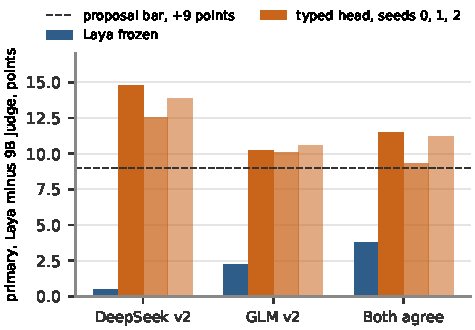
\includegraphics[width=0.5\linewidth]{figs/fig_typed_val.pdf}
\caption{Validation primary, Laya minus the 9B SLM judge, for the frozen design and the three typed head seeds (guide v2 labels). Every typed seed clears the proposal's 9 point bar on every label set.}\label{fig:typedval}
\end{figure}

\section{Evaluations}\label{sec:eval}
\subsection{Task accuracy and cost on test}\label{sec:eval-live}
\begin{figure}[H]
\centering
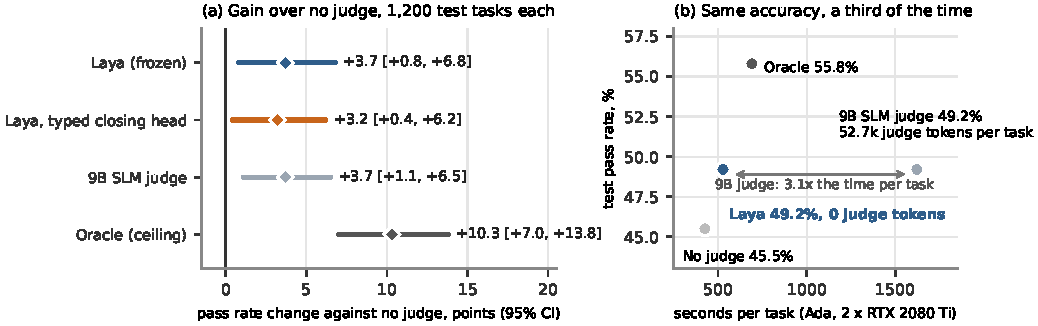
\includegraphics[width=\linewidth]{figs/fig_live_test.pdf}
\caption{Live test, Qwen3.5 9B agent, rollback plus done check, 1,200 tasks per system. (a) Pass rate change against no judge, paired bootstrap over the 100 test scenarios. The typed head is compared with the no judge passes on the same rented GPU, the other rows with the Ada no judge run. (b) Pass rate against time per task on Ada.}\label{fig:live}
\end{figure}

\begin{table}[H]
\centering\tablestyle
\caption{Live test results by BFCL version (Ada, 1,200 tasks per system). Gains are paired over the 100 test scenarios.}\label{tab:live}
\begin{tabularx}{\linewidth}{Yrrrrrlrr}
\toprule
\textbf{System} & \textbf{Base} & \textbf{Miss.\ param} & \textbf{Miss.\ func} & \textbf{Long ctx} & \textbf{All} & \textbf{vs no judge} & \textbf{Judge tok.} & \textbf{s / task} \\
\midrule
No judge & 58.3 & 39.3 & 29.3 & 55.0 & 45.5 & & 0 & 426 \\
\textbf{Laya} & 63.3 & 39.7 & 32.7 & 61.0 & \textbf{49.2} & \textbf{+3.7 [+0.8, +6.8]} & \textbf{0} & \textbf{528} \\
9B SLM judge & 61.3 & 41.7 & 34.0 & 59.7 & 49.2 & +3.7 [+1.1, +6.5] & 52,672 & 1,621 \\
Oracle (ceiling) & 69.0 & 50.3 & 38.3 & 65.7 & 55.8 & +10.3 [+7.0, +13.8] & 0 & 691 \\
\midrule
Typed Laya (rented GPU) & 63.3 & 40.3 & 33.3 & 62.0 & 49.8 & +3.2 [+0.4, +6.2] & 0 & \\
\bottomrule
\end{tabularx}
\end{table}

\textbf{Laya gives the SLM judge's accuracy at a fraction of its cost.} Both checkers lift the pass rate by 3.7 points with the interval above zero, and Laya minus the judge is +0.0 [\m2.8, +2.9]. The lower end, \m2.8, is inside the proposal's 5 point margin, so Laya is as accurate as the judge. It spends no judge tokens against 52,672 per task, and needs 528 seconds per task against 1,621, a third of the time. Laya adds only 24\% to the time of the bare agent; the 9B judge adds 280\%. Laya is at or above no judge on all four versions, with the largest gains on long context (+6.0) and base (+5.0). Both checkers recover 36\% of the oracle's +10.3 using the same corrections. The typed head keeps the gain live (+3.2 [+0.4, +6.2]) while flagging more (3.17 against 1.99 corrections per task).

\subsection{Detection: primary metric on test}\label{sec:eval-primary}
\begin{figure}[H]
\centering
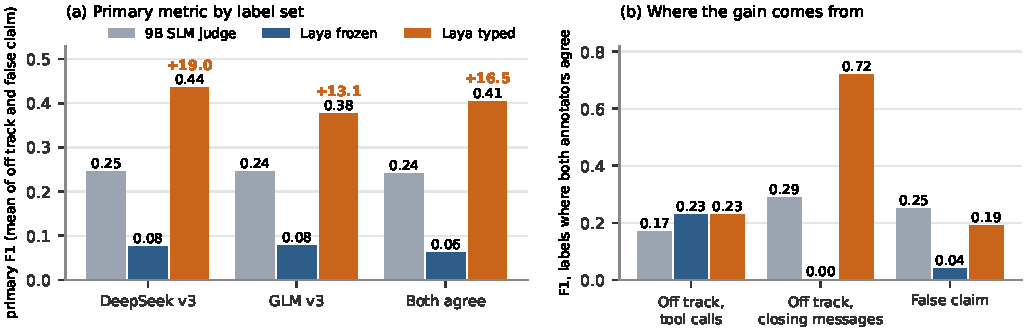
\includegraphics[width=\linewidth]{figs/fig_primary_test.pdf}
\caption{Primary metric on the 7,214 labelled test steps. (a) By label set; orange numbers are typed Laya minus the 9B judge, in F1 points. (b) Per class, on the steps where both annotators agree.}\label{fig:primary}
\end{figure}

\begin{table}[H]
\centering\tablestyle
\caption{Primary metric on test, guide v3 labels. Positives in brackets. Paired bootstrap over the 100 test scenarios. The typed head was built after the freeze; all its choices were fixed before training and test was scored once.}\label{tab:primary}
\begin{tabularx}{\linewidth}{lYccccc}
\toprule
\textbf{Labels} & \textbf{System} & \textbf{Off track} & \textbf{False claim} & \textbf{Primary} & \textbf{$-$ 9B [95\% CI]} & \textbf{$-$ Laya frozen} \\
\midrule
DeepSeek & 9B SLM judge & 0.25 (1,142) & 0.25 (91) & 0.246 & & \\
 & Laya frozen & 0.09 & 0.06 & 0.076 & \m17.0 [\m22.0, \m11.2] & \\
 & \textbf{Laya typed} & \textbf{0.63} & 0.24 & \textbf{0.436} & \textbf{+19.0 [+12.8, +24.8]} & +36.0 [+28.6, +42.5] \\
GLM & 9B SLM judge & 0.25 (1,015) & 0.24 (76) & 0.245 & & \\
 & Laya frozen & 0.10 & 0.06 & 0.078 & \m16.7 [\m22.0, \m10.4] & \\
 & \textbf{Laya typed} & \textbf{0.56} & 0.19 & \textbf{0.376} & \textbf{+13.1 [+7.7, +18.6]} & +29.8 [+23.6, +35.6] \\
Both agree & 9B SLM judge & 0.23 (775) & 0.25 (49) & 0.240 & & \\
 & Laya frozen & 0.08 & 0.04 & 0.063 & \m17.7 [\m23.7, \m10.4] & \\
 & \textbf{Laya typed} & \textbf{0.62} & 0.19 & \textbf{0.405} & \textbf{+16.5 [+9.9, +22.8]} & +34.2 [+26.7, +41.1] \\
\bottomrule
\end{tabularx}
\end{table}

\textbf{The typed head clears the proposal's bar.} Typed Laya beats the 9B judge by 13.1 to 19.0 F1 points under every label set, each estimate above the 9 point bar and each interval above zero. The gain comes from off track closing messages: F1 0.65 to 0.72 against 0.27 to 0.29 for the judge. On false claims, typed Laya (0.19 to 0.24) is close to the judge (0.24 to 0.25) without any reasoning. On tool calls, Laya's step head leads the judge on off track F1 under every label set (0.28 against 0.21, 0.25 against 0.21, 0.23 against 0.17).

\textbf{The frozen design, as pre-registered, does not meet the hypothesis.} It is 17 points below the judge. 980 of the 1,142 off track positives (DeepSeek) are closing messages, where a binary done head can never say off track, and the judge catches false claims far better on test (0.25) than on validation (0.05). Separating the closing message answer into three types removes the gap and turns it into a lead.

\subsection{Why the agent fails}\label{sec:eval-fail}
\begin{figure}[H]
\centering
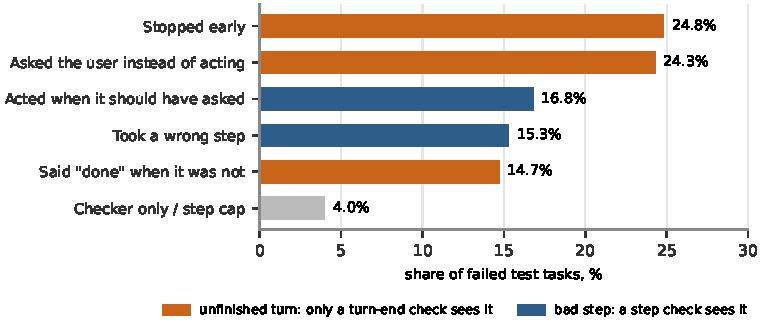
\includegraphics[width=0.62\linewidth]{figs/fig_failures.pdf}
\caption{Type of the first failed turn of each failed test task: 1,711 of the 3,200 no judge tasks, from the replay oracle.}\label{fig:failures}
\end{figure}
Most failures are unfinished turns: the agent stopped early (24.8\%), asked the user instead of acting (24.3\%) or said ``done'' when it was not (14.7\%). Only 32\% are bad steps that a step check can see: acting when it should have asked (16.8\%) and a wrong step (15.3\%). This is why the turn end check carries most of the gain, and why the typed head's off track class matters. When the agent is sent back, it often stops again. BFCL's scripted user gives no new information, so a bare ``not done, try again'' helps less than a specific hint would. Laya recovers 36\% of the oracle's gain by flagging alone. Going further means guiding, not just flagging: ``you forgot to send the email'' instead of ``not done''. The typed head is the first step, since it knows which kind of problem it saw.

\subsection{Label quality}\label{sec:annot}
\begin{figure}[H]
\centering
\begin{minipage}{0.44\linewidth}
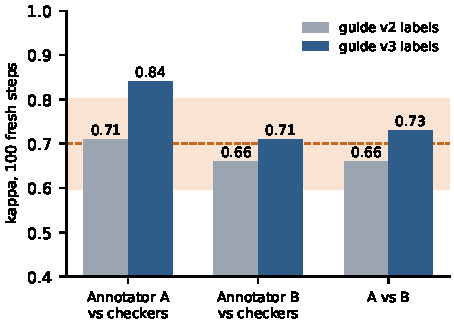
\includegraphics[width=\linewidth]{figs/fig_kappa.pdf}
\end{minipage}\hfill
\begin{minipage}{0.53\linewidth}
\caption{LLM annotators against the human consensus on a fresh sample of 100 validation steps, kappa reweighted to the real mix. The shaded band is the proposal's ``label more steps'' range, the dashed line the 0.7 bar. Guide v3 was written from a separate 100 step pilot, so the fresh sample is the fair test.}\label{fig:kappa}
\end{minipage}
\end{figure}
Swayam and Aaditya each labelled 200 sampled validation steps blind, half flagged by the annotators, and Pavan refereed their disagreements. After one guide rewrite, the annotators reach kappa 0.84 (A) and 0.71 (B) against the human consensus. A reaches the proposal's top band (above 0.8) and B the 0.7 bar. On the 7,214 test steps, the two annotators agree on 97.0\% of tool calls (kappa 0.57), 75.8\% of closing messages over the three scored classes (kappa 0.55), and 96.7\% on false claims (kappa 0.57). Every result is reported against each annotator separately and where both agree, and the conclusions hold under all three.

\section{Limitations}\label{sec:limits}
\begin{itemize}
  \item \textbf{The typed head is a change after the freeze.} Its choices were fixed before training and test was scored once, but it was designed after the frozen design's validation diagnosis. Confirming the primary hypothesis needs fresh test data. The pre-registered frozen design does not meet it.
  \item \textbf{Training and test labels share annotators.} The typed head trained on labels from the same two annotators that grade test (guide v3, train scenarios only), while the frozen heads trained on the oracle.
  \item \textbf{Labels are LLM labels.} The human check covers 200 validation steps. The planned 100 step human check of test steps and the test F1 reweighted to the real mix of turns were not done (the sample over-weights failed turns, by the proposal's rule). Annotator agreement on test is kappa 0.55 to 0.57. Eight passes gave 49 to 91 false claim positives in the test sample, short of the 300 targeted, so the false claim half has wider intervals than the off track half (775 to 1,142 positives).
  \item \textbf{One benchmark, one agent for the main claim.} BFCL has known flawed tasks, and its scripted user gives no new information when asked. AgentDojo results use the Qwen3 8B agent only.
  \item \textbf{Hardware differs between runs.} The Ada live runs (two RTX 2080 Ti, fp16, vLLM 0.19.1) and the rented GPU runs (bf16, vLLM 0.27.1) are each compared only with a no judge run from the same setup.
  \item \textbf{Not run:} confidence-gated escalation to the SLM judge, calibration, the state part ablation (no plan, no recent calls, no evidence list), AgentProcessBench and AgentHallu, the Gemma 4 12B reference judge~\cite{gemma}, directed error runs with a 27B model, and a guide v3 relabel of all validation steps.
\end{itemize}

\section{Conclusions}\label{sec:conclusion}
A 0.4B classifier can replace a reasoning 9B judge inside a small local agent. On 1,200 held out BFCL tasks, Laya gives the same +3.7 point gain as the 9B judge, at zero judge tokens and a third of the time per task. On detection, the decisive design choice is the closing message. A capable small agent fails mostly by leaving turns unfinished, not by taking wrong steps. A binary done head misses those turns under the proposal's scoring and falls 17 points short of the judge. A typed head that separates ``forgot a step'' from ``false claim'' beats the judge by 13 to 19 F1 points on the same test steps. Finetuning matters: off the shelf, every small judge we tried blocked almost everything.

\textbf{Future work.} (1) Confirm the typed head on fresh test passes. (2) Turn its typed answer into specific guidance for the agent, the most direct route to more of the oracle's +10.3 points. (3) Confidence-gated escalation of uncertain steps to the SLM judge. (4) Outside benchmarks with multi app tasks, such as AppWorld, and step-labelled sets such as AgentProcessBench.

\section{Team}
\begin{table}[H]
\centering\tablestyle
\caption{Main work of each member. All four wrote and revised the proposal.}\label{tab:roles}
\begin{tabularx}{\linewidth}{P{0.16\linewidth}Y}
\toprule
\textbf{Shuban Biswas} & Harness and replay oracle. Qwen3 8B baselines on BFCL test and AgentDojo, Qwen3 8B and Qwen3.5 4B validation runs, correction action study, offline scorer for off the shelf judges and plain rules. \\
\textbf{Ch Pavan Harshit} & Qwen3.5 9B agent runs, LLM annotation runs, Laya finetuning of the step and done heads, live checks and primary metric analysis, the 8 test passes, test labels and 9B judge on the rented GPU, the typed closing message head and its live run, referee of the human check. \\
\textbf{Swayam Goyal} & Human check of the LLM annotations (with Aaditya), annotation guide v3, Gate 1 counts, step head seeds and threshold cross validation on Ada, the frozen heads, Laya on the Qwen3 8B test, and the live 9B test runs on Ada. \\
\textbf{Aaditya Sharma} & Human check of the LLM annotations (with Swayam), review of disagreements by error type, final report and figures. \\
\bottomrule
\end{tabularx}
\end{table}

\section{Reproducibility and repository}\label{sec:repo}
\url{https://github.com/ch-pavan/lma-grp-project} holds all code, data and results, with a top level \code{README.md} that gives the setup and the command for every table and figure. Key folders: \code{shuban\_findings/} (harness, baselines, offline scorer), \code{analysis/} (oracle and step labels, annotation, Laya training and scoring, write ups), \code{human\_check/} (guides, samples, sheets, results), \code{runs/} (run outputs, labels, Laya datasets, GPU job scripts for Turing, Ada and the rented GPU) and \code{final\_report/} (this report, its figures and the number-to-source map). Laya weights are on the GitHub releases \code{laya-heads-frozen-2026-11-08} and \code{laya-typed-head-2026-11-09}.

{\footnotesize
\begin{tabular}{@{}ll@{}}
\code{python analysis/rb\_test\_results.py} & live test results (Table~\ref{tab:live}) \\
\code{python analysis/live\_compare.py} & typed head live result \\
\code{python analysis/primary\_test.py} & primary metric on test (Table~\ref{tab:primary}) \\
\code{python analysis/oracle\_labels.py runs/raw/test9b/test} & failure types on test (Figure~\ref{fig:failures}) \\
\code{python analysis/primary\_val.py} & primary metric on validation \\
\code{python human\_check/score.py human\_check/val2 -{}-guide v3} & annotation check (Figure~\ref{fig:kappa}) \\
\code{python final\_report/scripts/test\_agreement.py} & annotator agreement on test \\
\code{python final\_report/scripts/live\_cost.py} & live cost and per version results \\
\end{tabular}}

\begin{thebibliography}{99}
\setlength{\itemsep}{0pt}\small
\bibitem{critictool} CRITICTOOL: evaluating self critique of LLMs in tool calling error scenarios. arXiv 2506.13977.
\bibitem{realtime} Real time detection and repair of LLM agent failures. arXiv 2608.02464.
\bibitem{agenthallu} AgentHallu: benchmarking automated hallucination attribution of LLM based agents. arXiv 2601.06818.
\bibitem{stepguard} StepGuard: learning step level guardrails. arXiv 2608.24777.
\bibitem{sentry} SAFETY SENTRY: context aware human intervention via execute, ask, refuse routing. arXiv 2607.13594.
\bibitem{agentdog} AgentDoG: a diagnostic guardrail framework for AI agent safety and security. arXiv 2601.18491.
\bibitem{granite} Granite Guardian. arXiv 2412.07724, with its 3.2 3B A800M model card.
\bibitem{minicheck} MiniCheck: efficient fact checking of LLMs on grounding documents. arXiv 2404.10774.
\bibitem{hhem} Vectara HHEM 2.1, model card. huggingface.co/vectara/hallucination\_evaluation\_model.
\bibitem{lettuce} LettuceDetect: hallucination detection for RAG. arXiv 2502.17125.
\bibitem{llamafirewall} LlamaFirewall and PromptGuard 2. arXiv 2505.03574.
\bibitem{toolrm} ToolRM: outcome reward models for tool calling LLMs. arXiv 2509.11963.
\bibitem{agentprm} AgentPRM: process reward models for LLM agents. arXiv 2511.08325.
\bibitem{layabrowser} laya browser, Laya step decision head for a browser agent. huggingface.co/cklxx/laya-browser.
\bibitem{laya} Laya typed decision model, model card. huggingface.co/convaiinnovations/laya.
\bibitem{zheng2023judge} L.\ Zheng et al. Judging LLM as a judge with MT Bench and Chatbot Arena. arXiv 2306.05685.
\bibitem{qwen} Qwen3.5 9B and 4B, model cards. huggingface.co/Qwen.
\bibitem{modernbert} ModernBERT: a modern bidirectional encoder. arXiv 2412.13663.
\bibitem{typesafe} TypeSafe, Jev and System One models. docs.typesafe.ai.
\bibitem{frugalgpt} L.\ Chen et al. FrugalGPT: how to use large language models while reducing cost and improving performance. arXiv 2305.05176.
\bibitem{bfcl} S.\ Patil et al. The Berkeley Function Calling Leaderboard (BFCL). ICML 2025.
\bibitem{bfclissues} BFCL answer key issues 1367, 1267, 1137 and 1377. github.com/ShishirPatil/gorilla.
\bibitem{agentdojo} AgentDojo. arXiv 2406.13352.
\bibitem{tau2} tau2 bench issue 384. github.com/sierra-research/tau2-bench.
\bibitem{mathshepherd} P.\ Wang et al. Math-Shepherd: verify and reinforce LLMs step by step without human annotations. arXiv 2312.08935.
\bibitem{agentprocessbench} AgentProcessBench: step level process quality in tool using agents. arXiv 2603.14465.
\bibitem{kev} Kev 0.8B, model card. huggingface.co/jaredpalmer/kev-0.8b.
\bibitem{when2call} When2Call: when (not) to call tools. arXiv 2504.18851.
\bibitem{gemma} Gemma 4 12B, release notes. ai.google.dev/gemma/docs/releases.
\bibitem{deepseek} DeepSeek V4.1 Flash, model card. huggingface.co/deepseek-ai.
\bibitem{baltes} S.\ Baltes et al. Guidelines for empirical studies in software engineering involving large language models. arXiv 2508.15503.
\bibitem{glm} GLM-5.3, model card. huggingface.co/zai-org.
\end{thebibliography}

\end{document}
